\chapter{Topics in scattering theory \label{chap:2}}

Light is in range of the electromagnetic spectrum where the wave-particle duality is most significant. This is the region where low energy radiation, described like waves, and high energy radiation, described like particles, come together. \\
Its interaction with matter is a complex phenomenon that can be addressed in different ways. Although the most precise description is given by the quantum electrodynamics, in nano-optics a big number of problems can be tackle by considering a semi-classical approach.\\
Usually is mostly sufficient the adoption of a wave picture to describe the optical radiation, allowing the use of classical field theory based on Maxwell equations.\\

In this chapter we start by presenting the Green function concept, Sec. (\ref{sec:chap2_dyadic_green_function}), which is the field generated by a point source, and the scattering of waves by small particles, in Sec. (\ref{sec:Wave_scatt_small_part}).\\
 In Sec. (\ref{chap:chap2_DDA}) introduce the Discrete Dipole Approximation to solve complex systems like irregular and big size particles or random structures.\\
In Sec. (\ref{sec:Pol_small_part}) we calculate the polarisability of small particles, in particular, small anisotropic spherical particles and its absorption.\\
In Sec. (\ref{sec:chap2_dielectric_tensor}) we discuss the properties of the dielectric tensor in the presence of a magnetic field and the formalism used to tackle magneto-optical problems.\\
Finally, in Sec. (\ref{chap2:Dipole_radiation}) is discussed the Purcell effect, by presenting some techniques to calculate the influence of the environment on an emitter.

\section{The Dyadic Green function\label{sec:chap2_dyadic_green_function}}

Maxwell's equations together with constitutive relations describe the fields generated by currents and charges in matter, as well as the behaviour of matter under the influence of fields \cite{Jackson_CE}.

In the frequency domain, for a non-magnetic medium, $\mu=1$, described by the dielectric permittivity $\varepsilon\left(\mathbf{r},\omega\right)$ and the sources by their current density $\mathbf{j}_{s}\left(\mathbf{r},\omega\right)$, the electric field in a linear, isotropic and inhomogeneous media should satisfy the wave equation:

\begin{equation}
\nabla\times\nabla\times\mathbf{E}\left(\mathbf{r},\omega\right) - k^2 \varepsilon\left(\mathbf{r},\omega\right)\mathbf{E}\left(\mathbf{r},\omega\right) = i\omega \mu_{0}\mathbf{j}_{s}\left(\mathbf{r},\omega\right),\label{eq:chap_2_wave_eq}
\end{equation}
where $k=\omega/c$ denotes the wavenumber in vacuum. The above equation carries information about the scattering elements in the system, which is represented by the second term of the left-hand side, while of the right-hand side term carries information about the sources.\\
Eq. (\ref{eq:chap_2_wave_eq}) is particularly difficult to solve for any type of source. An interesting case is the point dipole source, that can be seen as an oscillating current positioned at $\mathbf{r}'$. Mathematically, the point source can be defined by $\delta\left(\mathbf{r}-\mathbf{r}'\right)$, where it is zero everywhere, except at $\mathbf{r} = \mathbf{r}'$ where it diverges.\\
For this equation and for each component of $\mathbf{j}_{s}$ is possible to define a Green function as solution of Eq. (\ref{eq:chap_2_wave_eq}):

\begin{equation}
\nabla\times\nabla\times\mathbf{G}_{i}\left(\mathbf{r},\mathbf{r}',\omega\right) - k^2 \varepsilon\left(\mathbf{r},\omega\right)\mathbf{G}_{i}\left(\mathbf{r},\mathbf{r}',\omega\right) = \delta\left(\mathbf{r}-\mathbf{r}'\right)\mathbf{n}_{i},\label{eq:2}
\end{equation}
where $\mathbf{n}_{i}$ is the unit vector in the $i$ direction.
A general definition, in a compact form, of the Green function for the electric field is given by:

\begin{equation}
\nabla\times\nabla\times\mathbf{G}\left(\mathbf{r},\mathbf{r}',\omega\right) - k^2 \varepsilon\left(\mathbf{r},\omega\right)\mathbf{G}\left(\mathbf{r},\mathbf{r}',\omega\right) = \mathbb{I}\delta\left(\mathbf{r}-\mathbf{r}'\right),\label{eq:chap2_eq3}
\end{equation}
where $\mathbb{I}$ is the unit dyad. Each column of the $\mathbf{G}$ tensor corresponds to the field generated by a point source oriented along the cartesian axes. The first column corresponds to the field due to an emitter oriented in the $x-$direction, the second column corresponds to the $y-$direction and the third to the $z-$direction.

A source current with a complex shape can be constructed as a superposition of point currents. If we know the Green function $\mathbf{G}$, a particular solution of Eq. (\ref{eq:chap_2_wave_eq}) is:

\begin{equation}
\mathbf{E}\left(\mathbf{r},\omega\right) = i\omega \mu_{0}\int_V^{}\mathbf{G}\left(\mathbf{r},\mathbf{r}',\omega\right)\mathbf{j}_{s}\left(\mathbf{r}',\omega\right) dV'.
\end{equation}
Adding the homogeneous solutions $\mathbf{E}_{0}$, the general solution, called volume integral equation, is given by:

\begin{equation}
\mathbf{E}\left(\mathbf{r},\omega\right) = \mathbf{E}_{0}\left(\mathbf{r}\right) +  i\omega \mu_{0}\int_V^{}\mathbf{G}\left(\mathbf{r},\mathbf{r}',\omega\right)\mathbf{j}\left(\mathbf{r}',\omega\right) dV' \qquad \mathbf{r} \notin V,
\end{equation}
and the corresponding magnetic field:

\begin{equation}
\mathbf{H}\left(\mathbf{r},\omega\right) = \mathbf{H}_{0}\left(\mathbf{r},\omega\right) +  \int_V^{}\left[\nabla \times \mathbf{G}\left(\mathbf{r},\mathbf{r}',\omega\right)\right]\mathbf{j}\left(\mathbf{r}',\omega\right) dV' \qquad \mathbf{r} \notin V.
\end{equation}
To avoid the singularity, the volume integral equations are limited to outside of the source.\\
%These are the fundamental equations that lies behind of coupled dipole method or the Lippmann-Schwinger equation.\\
For the three dimensional space, the dyadic Green function $\mathbf{G}$ reads:

\begin{equation}
\mathbf{G}\left(\mathbf{r},\mathbf{r}',\omega\right) = \frac{e^{ikR}}{4\pi R}\left[\left(1+\frac{ikR-1}{k^2R^2}\right)\mathbb{I}+\frac{3-3ikR-k^2R^2}{k^2R^2}\frac{\mathbf{R} \otimes\mathbf{R}}{R^2}\right],\label{Green_tensor}
\end{equation}
where $\mathbf{R} = \mathbf{r} - \mathbf{r}'$ and $R$ is its modulus.\\
In the Green function $\mathbf{G}$ it is possible to identify three different terms, $\left(kR\right)^{-1}$, $\left(kR\right)^{-2}$ and $\left(kR\right)^{-3}$. In the near field, when $R\ll\lambda$, the term $\left(kR\right)^{-3}$ dominates. In the far field, for which $R\gg\lambda$, the dominant term is $\left(kR\right)^{-1}$. For the intermediate field, when $R\approx\lambda$, the three elements are relevant.

Physically the Green tensor $\mathbf{G}$  connects the field $\mathbf{E}$ at some position $\mathbf{r}$, generated by a point dipole emitter $\boldsymbol{\mu}$ at position $\mathbf{r}'$. The current density that generates such a source is
$\mathbf{j}\left(\mathbf{r}\right) = -i\omega \boldsymbol{\mu} \delta \left(\mathbf{r}-\mathbf{r}'\right)$, and the electric field can be mathematically expressed as:

\begin{equation}
\mathbf{E}\left(\mathbf{r},\omega\right) = \frac{k^2}{\epsilon_{0}}\mathbf{G}\left(\mathbf{r},\mathbf{r}',\omega\right)\boldsymbol{\mu}.\label{eq:EM_source}
\end{equation}

\section{Wave scattering by small particles\label{sec:Wave_scatt_small_part}}

When light propagates through an inhomogeneous medium, some constituent elements, like particles, can be excited and behave like secondary sources. The new sources, with size much smaller than the incident wavelength, get polarised when illuminated.\\
In general, it is possible to define the electromagnetic field over a particle as a sum of two excitation fields, the incident field, $\mathbf{E}_{0}$, and the scattered field, $\mathbf{E}_s$:

\begin{equation}
\mathbf{E}\left(\mathbf{r},\omega\right) = \mathbf{E}_{0}\left(\mathbf{r},\omega\right) + \mathbf{E}_s\left(\mathbf{r},\omega\right). \label{eq:fields}
\end{equation}

In free space and in the absence of any particle, the electric field obeys the free-space propagation equation:

\begin{equation}
\nabla \times \nabla \times \mathbf{E}_{0}\left(\mathbf{r,\omega}\right) - k^2 \mathbf{E}_{0}\left(\mathbf{r,\omega}\right) = 0. \label{eq:wa_eq_totfield}
\end{equation}

We can describe the particle as a modification of the dielectric tensor at some position. It can be written as  $\boldsymbol{\epsilon}\left(\mathbf{r},\omega\right) = 1+\Theta\left(a-\left|\mathbf{r}-\mathbf{r}_p\right|\right)\left[\boldsymbol{\epsilon}\left(\omega\right)-1\right]$, being $\Theta$ the Heaviside step function which is $0$ everywhere except inside of the particle. For the sake of brevity we going to write $\Theta\left(a-\left|\mathbf{r}-\mathbf{r}_p\right|\right)$ only as $\Theta$.\\
The total electric field can be obtained by solving the wave equation:

\begin{equation}
\nabla \times \nabla \times \mathbf{E}\left(\mathbf{r,\omega}\right) - k^2 \left\{ \mathbb{I} + \Theta \right[\boldsymbol{\epsilon}\left(\omega\right) - \mathbb{I}\left]\right\}\mathbf{E}\left(\mathbf{r}, \omega\right) = 0,\label{eq:wa_eq_incfield}
\end{equation}

%To obtain the propagation equation of the scattered field, we subtract Eq. (\ref{eq:wa_eq_totfield}) to Eq. (\ref{eq:wa_eq_incfield}):
which can be expressed in the form:


\begin{equation}
\nabla \times \nabla \times \mathbf{E}\left(\mathbf{r,\omega}\right) - k^2 \mathbf{E}\left(\mathbf{r}, \omega\right) = k^2\Theta\left[\boldsymbol{\epsilon}-\mathbb{I}\right]\mathbf{E}\left(\mathbf{r},\omega\right).\label{eq:wa_eq_finfield}
\end{equation}

%Eq. (\ref{eq:wa_eq_finfield}) is a propagation equation in vacuum, where the source term is proportional to the total electric field. This equation is very similar with Eq. (\ref{eq:chap2_eq3}), where the source element is a point in space. 
The solution of this equation can then be expressed in terms of the Green function $\mathbf{G}$:

%\begin{equation}
%\mathbf{E}_{s}\left(\mathbf{r},\omega\right) =  k^{2}\left[\boldsymbol{\epsilon}\left(\omega\right) -\mathbb{I}\right] \int_{V'}{\mathbf{G}\left(\mathbf{r},\mathbf{r}',\omega\right)}\mathbf{E}\left(\mathbf{r}',\omega\right)dV', \label{eq:wa_sca}
%\end{equation}
%
%where the prime in $V'$ indicates that the integration refers to $\mathbf{r}'$.
%
%The total field at position $\mathbf{r}$ is obtained by substituting Eq. (\ref{eq:wa_sca}) in Eq. (\ref{eq:fields}):

\begin{equation}
\mathbf{E}\left(\mathbf{r},\omega\right) =  \mathbf{E}_{0}\left(\mathbf{r},\omega\right) + k^{2}\left[\boldsymbol{\epsilon}\left(\omega\right) -\mathbb{I}\right] \int_{V'}{\mathbf{G}\left(\mathbf{r},\mathbf{r}_{p},\omega\right)}\mathbf{E}\left(\mathbf{r}_p,\omega\right)dV', \label{eq:lipschw}
\end{equation}
obtaining the so-called Lippmann-Schwinger equation \cite{Martin_1994}.\footnote{Usually referred in literature as volume integral equation.}

Here we should note that Eq. (\ref{eq:wa_eq_finfield}) as the same form as Eq. (\ref{eq:chap_2_wave_eq}) with the source term:

\begin{equation}
\mathbf{j}_s\left(\mathbf{r},\omega\right) = -\frac{i}{\omega \mu_{0}\mu}k^3\Theta\left[\boldsymbol{\epsilon}-\mathbb{I}\right]\mathbf{E}\left(\mathbf{r},\omega\right).
\end{equation}


\section{Discrete Dipole Approximation\label{chap:chap2_DDA}}

An important problem in nanophotonics is the modification of the electromagnetic field distributions and the associated radiation properties by complex structures. Due to the complexity of such problems, it is not possible to obtain analytical solutions of Maxwell's equations. Different approaches can be considered, that can go from pure numerical (like finite-difference time-domain or finite-element methods) to semi-analytical techniques (like volume integral method). We consider the semi-analytical approach, a particular implementation of the volume integral method is called Discrete Dipole Approximation\footnote{Also called Coupled Dipole Approximation.} (DDA).\\
Introduced by DeVoe \cite{devoe1964optical} in 1964 and improved by Purcell and Pennypacker \cite{Purcell_1973} in 1973, the DDA has been applied in many different problems, that go from interstellar dust grains \cite{draine1988discrete} to biological tissues \cite{yurkin2005experimental}. Roughly speaking, the DDA is an approximation of the continuum target by a finite number of polarisable points. The dipoles interact with one another via their electric field.\\
The method is a flexible and powerful technique to compute the scattering and absorption by irregular and relatively big size particles \cite{draine1988discrete, draine1994discrete, draine2008discrete} or complex structures like random systems \cite{Froufe_PRA_2007}. It allow us to solve Maxwell's equations exactly, taking into account retardation and near-field interactions, the multiple scattering and the polarisation.\\
For big and irregular particles, the volume is discretised into point dipoles, schematically presented in Fig. (\ref{fig:chap2_DDA_scheme})(a). The only approximation is the replacement of the continuum target by an array of point dipoles. In random systems each particle is described as a single dipole, that interacts with all others present in the system, as shown in Fig. (\ref{fig:chap2_DDA_scheme})(b). In this case the approximation is in the description of the particle as a single dipole. Both cases can be mixed, \textit{i.e.}, we can describe particles formed by many dipoles that interact with other particles with the same formalism.  
For its application, a fundamental condition has to be fulfilled: the point dipoles represent volume elements or particles sufficiently small to neglect any variation of the electromagnetic field inside its volume.

\begin{figure}[h]
\begin{centering}
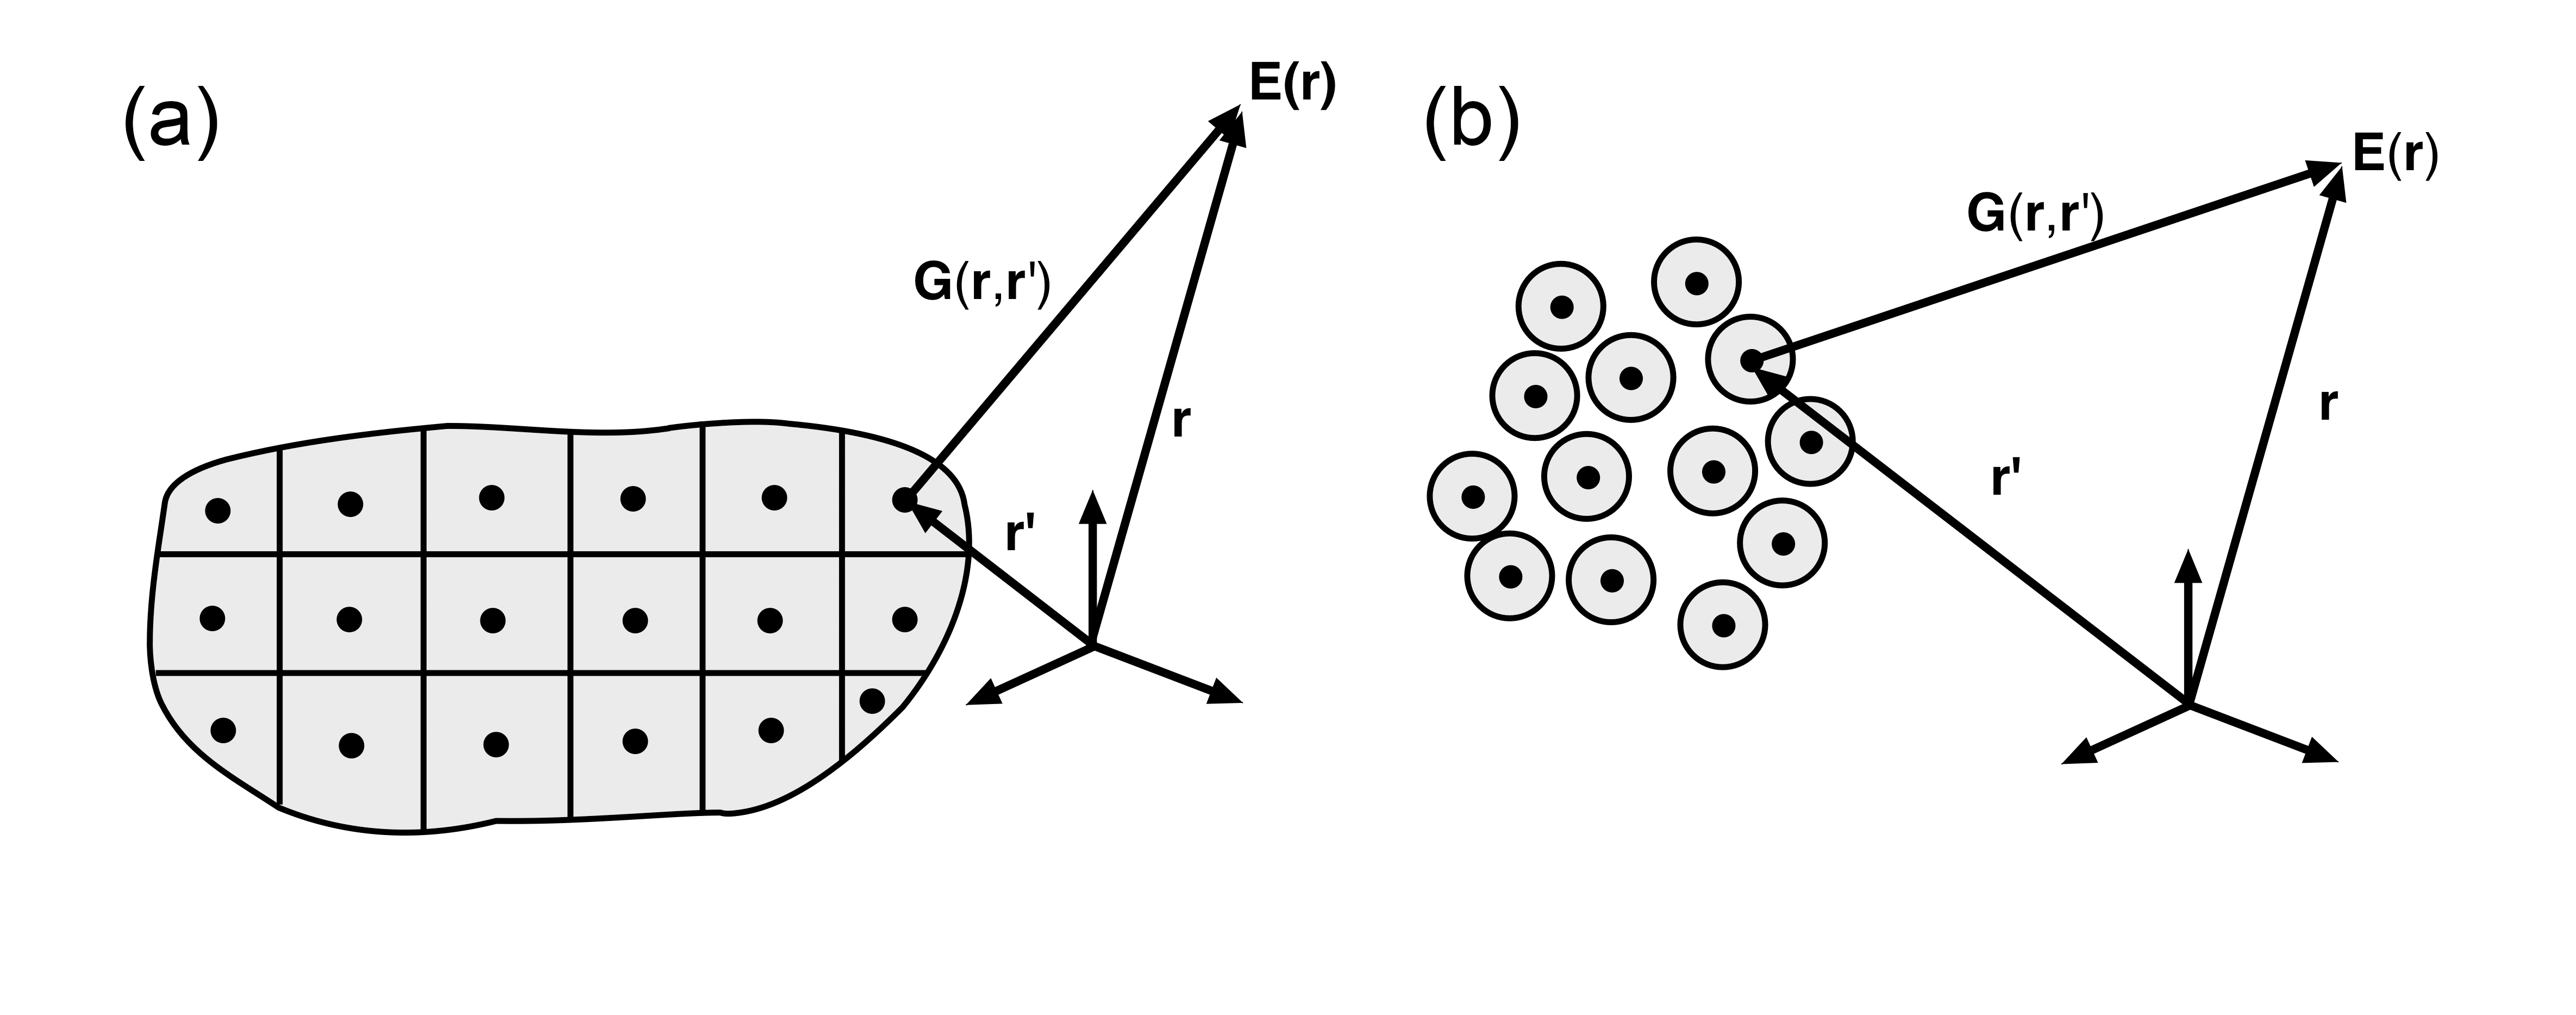
\includegraphics[width=10cm]{chapter_2/figures/DDA.png} 
\par\end{centering}
\caption{Schematic representation of: (a) a discretised object into dipoles (black points); (b) a random systems where each particle is described by a single dipole. The electric field $\mathbf{E}$ at point $\mathbf{r}$, in both situations, is obtained from the sum of the field from each dipole. \label{fig:chap2_DDA_scheme}}
\end{figure}
For a set of $\mathcal{N}$ dipoles which form a system, the excitation field over each dipole can be obtained by considering Eq. (\ref{eq:lipschw}) in the discrete form:

\begin{equation}
\mathbf{E}_{i} =  \mathbf{E}_{0}\left(\mathbf{r}_i,\omega\right) + \frac{k^2}{\epsilon_{0}}\sum_{i\neq j}{\mathbf{G}\left(\mathbf{r}_i,\mathbf{r}_j,\omega\right)}\epsilon_{0}\boldsymbol{\alpha}\mathbf{E}_{j},\label{eq:chap2_DDA}
\end{equation}
where $\mathbf{p}_i=\epsilon_{0}\boldsymbol{\alpha}\mathbf{E}_i$ is the induced dipole moment or the polarisation\footnote{We describe the polarisation of particles in chapter (\ref{chap2:pol_of_small_particles}).} of the $i-$element. Eq. (\ref{eq:chap2_DDA}) is a set of $3\mathcal{N}$ linear equations with $3\mathcal{N}$ unknowns, representing the exciting fields at the scatterer's position. Solving the system of equations, it is possible to know the polarisation of each dipole, which in turn allows us to obtain the electric field at any position in the space:

\begin{equation}
\mathbf{E}\left(\mathbf{r},\omega\right) =  \mathbf{E}_{0}\left(\mathbf{r},\omega\right) + \frac{k^2}{\epsilon_{0}}\sum_{i=1}^{\mathcal{N}}{\mathbf{G}\left(\mathbf{r},\mathbf{r}_{i},\omega\right)}\epsilon_{0}\boldsymbol{\alpha}\mathbf{E}_{i}.
\end{equation}

\section{Polarisability of small particles\label{sec:Pol_small_part}}

The result of light interaction with matter depends not only of light properties (frequency, intensity, etc.) but also the matter properties (dielectric response, shape, etc.).\\
This section is devoted to the study of the electromagnetic response of small particles, when compared with the incident wavelength, when illuminated. 
Small particles get polarised when excited, exhibiting an induced dipole. This behaviour allow us to regard each particle as a new source of radiation, commonly referred as a secondary source (see Sec. \ref{sec:Wave_scatt_small_part}). 

Let us consider a small particle in vacuum with volume $V$ and with dielectric tensor $\boldsymbol{\epsilon}\left(\omega\right)$. The particle is positioned at $\mathbf{r}_p$ and the incident electric field that excites the particle is $\mathbf{E}_{0}\left(\omega\right)$. The polarisability $\boldsymbol{\alpha}$ of the particle relates the incident electric field $\mathbf{E}_{0}\left(\omega\right)$ with the polarisation $\mathbf{p}\left(\omega\right)$. Mathematically, can be represented as:

\begin{equation}
\mathbf{p}\left(\omega\right) = \epsilon_{0}\boldsymbol{\alpha}\left(\omega\right) \mathbf{E}_{0}\left(\omega\right).
\end{equation}

The polarisability takes into account the shape and dimensions as well as the electromagnetic response of the particle material. Its anisotropic nature implies that the induced dipole can have an orientation which is different from the incident electric field.
% a different orientation of the incident electric field. 
In the following subsection we calculate the polarisability for small anisotropic spherical particles.

\subsection{Polarisability of small anisotropic spherical particles\label{chap2:pol_of_small_particles}}

Let us consider a single spherical particle with radius $a$, much smaller than the wavelength, where the electric field does not vary inside of its volume. \\
From the Lippmann-Schwinger equation, we can approximate the total electric field for a point $\mathbf{r}$ outside of the particle:

\begin{equation}
\mathbf{E}\left(\mathbf{r}\right) \approx \mathbf{E}_{0}\left(\mathbf{r}\right) + k^{2}\left[\boldsymbol{\epsilon}-\mathbb{I}\right]V\mathbf{G}\left(\mathbf{r},\mathbf{r}_{p}\right)\mathbf{E}_{ins}\label{eq:chap2:E_tot_comp},
\end{equation}
where $\mathbf{E}_{ins}$ is the electric field inside the particle. Because the particle is the only scatterer present in the system, the electric field that illuminates the particle is $\mathbf{E}_{0}\left(\mathbf{r}_{p}\right)$. The particle's dipole can be written as:

\begin{equation}
\mathbf{p}=\epsilon_0\boldsymbol{\alpha}\mathbf{E}_{0}\left(\mathbf{r}_{p}\right).
\end{equation}
Eq. (\ref{eq:chap2:E_tot_comp}) can be rewritten in a more compact way:

\begin{equation}
\mathbf{E}\left(\mathbf{r}\right) \approx \mathbf{E}_{0}\left(\mathbf{r}\right) + \frac{k^2}{\epsilon_{0}}\mathbf{G}\left(\mathbf{r},\mathbf{r}_{p}\right)\mathbf{p}.
\end{equation}
In this approximation we can use Eq. (\ref{eq:lipschw}) to obtain the self-consistent solution for $\mathbf{E}_{ins}$:

\begin{eqnarray}
\mathbf{E}_{ins} & = & \mathbf{E}_{0}\left(\mathbf{r}_{p}\right)+k^{2}\left[\boldsymbol{\epsilon}-\mathbb{I}\right]\left(\int \mathbf{G}\left(\mathbf{r},\mathbf{r}_{p}\right)dV'\right)\cdot\mathbf{E}_{ins}\nonumber \\
 & = & \mathbf{E}_{0}\left(\mathbf{r}_{p}\right)+k^2\left[\boldsymbol{\epsilon}-\mathbb{I}\right]V\left<\mathbf{G}\right>\cdot\mathbf{E}_{ins},
\end{eqnarray}
where $\left<\mathbf{G}\right>$  is the average value of the Green tensor in the volume of the particle $V$ which came from the volume integral.\\
The internal self-consistent field is given by:

\begin{equation}
\mathbf{E}_{ins} = \left\{\mathbb{I}-k^2V\left<\mathbf{G}\right>\left[\boldsymbol{\epsilon}-\mathbb{I}\right]\right\}^{-1}\mathbf{E}_{0}\left(\mathbf{r}_{p}\right).
\end{equation}

For small spherical particles, the average Green tensor is given by \cite{Bladel_1961, Yaghjian_1980,Wang_1991,Carminati_2006}:

\begin{equation}
\lim_{v\rightarrow 0}\left<\mathbf{G}\right>\simeq \left(-\frac{1}{3k^2V}+i\frac{k}{6\pi}\right)\mathbb{I},
\end{equation}
where $\Im\left\{\mathbf{G}\left(0\right)\right\}=\frac{k}{6\pi}\mathbb{I}$.
So, we have:

\begin{equation}
\mathbf{E}_{ins} = \left[\mathbb{I}+\left(\frac{1}{3}-\frac{ik^3V}{6\pi}\right)\mathbb{I}\left(\boldsymbol{\epsilon}+2\mathbb{I}\right)\right]^{-1}\mathbf{E}_{0}\left(\mathbf{r}_{p}\right).
\end{equation}


Defining $\boldsymbol{\alpha}_0 = 3V\left\{\boldsymbol{\epsilon}-\mathbb{I}\right\}\left\{\boldsymbol{\epsilon}+2\mathbb{I}\right\}^{-1}$ as the static polarisability, it is possible to express the field inside as:

\begin{equation}
\mathbf{E}_{ins}=3\left(\boldsymbol{\epsilon}+2\mathbb{I}\right)^{-1}\left\{\mathbb{I}-i\frac{k^3}{6\pi}\boldsymbol{\alpha}_{0}\right\}^{-1}\mathbf{E}_{0}\left(\mathbf{r}_{p}\right).\label{eq:field_inside_particle}
\end{equation}
The total field outside of the particle can be expressed as:

\begin{eqnarray}
\mathbf{E}\left(\mathbf{r}\right) & = & \mathbf{E}_{0}\left(\mathbf{r}\right)+k^{2}\int\mathbf{G}\left(\mathbf{r},\mathbf{r}_{p}\right)\left(\boldsymbol{\epsilon}-\mathbb{I}\right)\mathbf{E}\left(\mathbf{r}'\right)dV' \nonumber \\
 & = & \mathbf{E}_{0}\left(\mathbf{r}\right)+k^{2}V\mathbf{G}\left(\mathbf{r},\mathbf{r}_{p}\right)\left(\boldsymbol{\epsilon}-\mathbb{I}\right)\mathbf{E}_{ins}\nonumber \\
 & = & \mathbf{E}_{0}\left(\mathbf{r}\right)+k^{2}V\mathbf{G}\left(\mathbf{r},\mathbf{r}_{p}\right)\left(\boldsymbol{\epsilon}-\mathbb{I}\right)3\left(\boldsymbol{\epsilon}+2\mathbb{I}\right)^{-1}\left\{\mathbb{I}-i\frac{k^3}{6\pi}\boldsymbol{\alpha}_{0}\right\}^{-1}\mathbf{E}_{0}\left(\mathbf{r}_{p}\right)\nonumber\\
 & = & \mathbf{E}_{0}\left(\mathbf{r}\right) + \frac{k^2}{\epsilon_{0}}\mathbf{G}\left(\mathbf{r},\mathbf{r}_{p}\right)\cdot \mathbf{p} \label{eq:chap2_poleq2}.
\end{eqnarray}
The induced dipole  $\mathbf{p}$ is obtained from the previous equations:

\begin{equation}
\boldsymbol{\alpha}\mathbf{E}_{0}\left(\mathbf{r}_{p}\right) = V\left(\boldsymbol{\epsilon}-\mathbb{I}\right)3\left(\boldsymbol{\epsilon}+2\mathbb{I}\right)^{-1}\left\{\mathbb{I}-i\frac{k^3}{6\pi}\boldsymbol{\alpha}_{0}\right\}^{-1}\mathbf{E}_{0}\left(\mathbf{r}_{p}\right),
\end{equation}
Substituting $\boldsymbol{\alpha}_0= 3V\left(\boldsymbol{\epsilon}-\mathbb{I}\right)\left(\boldsymbol{\epsilon}+2\mathbb{I}\right)^{-1}$ we obtain:

\begin{equation}
\boldsymbol{\alpha}=\boldsymbol{\alpha}_{0}\left\{\mathbb{I}-i\frac{k^3}{6\pi}\boldsymbol{\alpha}_{0}\right\}^{-1}\label{eq:chap2_radiative_correction}.
\end{equation}
Eq. (\ref{eq:chap2_radiative_correction}) is the expression of the polarisability with the radiative correction, that is valid for any permittivity tensor $\boldsymbol{\epsilon}$.

\subsection{Polarisability of resonant particles\label{sec:chap2_resonant}}

Resonant point dipoles are special particles because they have the ability of maximise the scattering of light. Is frequently used in theoretical models where phenomena are critical with the amount of scattering.\\
For a resonant particle, is considered a diagonal dielectric tensor only with real part, \textit{i.e.}, without absorption, where the static polarisability is maximum. The diagonal elements of the dielectric tensor assume the value of $\epsilon = -2$ for a given frequency. Thus, the resonant polarisability with radiative corrections for a spherical particle is given by:

\begin{equation}
\alpha_{res} = i\frac{6\pi}{k^3}.
\end{equation}

\subsection{Absorption of small particles\label{sec:chap2_abs_small_part}}

When light is incident over a particle, a fraction of the incident beam can be absorbed and transformed into internal energy, usually in thermal energy \cite{Baffou_2009}.
In this section we evaluate the absorbed power by a small particle.\\
The mean of energy absorbed, over a period, within the volume $V$ is given by:

\begin{equation}
\left<\frac{dW_{abs}}{dt}\right>=\frac{1}{2}\int_{V}\Re\left\{\mathbf{j}^{*}\cdot\mathbf{E}_{ins}\right\}dV,\label{eq:mean_energy_absorbed}
\end{equation}
where $\mathbf{j}=-i\omega \mathbf{p}\delta\left(\mathbf{r}-\mathbf{r}'\right)$ is the current induced by the field inside the particle $\mathbf{E}_{ins}$. Eq. (\ref{eq:mean_energy_absorbed}) can be written as:

\begin{equation}
\left<\frac{dW_{abs}}{dt}\right>=P_{abs}=-\frac{\omega}{2} \Im\left\{\mathbf{p}^{*}\cdot\mathbf{E}_{ins}\right\}.
\end{equation}
The electric field inside of the particle is defined by Eq. (\ref{eq:field_inside_particle}) and the dipole moment of the particle can be expressed as:

\begin{equation}
\mathbf{p} = V\epsilon_{0}\left(\boldsymbol{\epsilon}-\mathbb{I}\right)\cdot\mathbf{E}_{ins},
\end{equation}
where can we get the absorbed power by the particle:

\begin{equation}
P_{abs} = -V\frac{\omega \epsilon_0}{2}\Im{\left\{\left(\boldsymbol{\epsilon}\cdot\mathbf{E}_{ins}\right)^{*}\cdot\mathbf{E}_{ins}\right\}}.\label{eq:abs_gen}
\end{equation}
For the special case where the dielectric tensor is diagonal, $\boldsymbol{\epsilon}=\epsilon\mathbb{I}$, Eq. (\ref{eq:abs_gen}) can be simplified:

\begin{equation}
P_{abs} = V\frac{\omega \epsilon_0}{2}\Im{\left\{\epsilon\right\}}\left|\mathbf{E}_{ins}\right|^2.\label{eq:Pabs_diel_cnst}
\end{equation}
To obtain the expression involving the polarisability, we substitute Eq. (\ref{eq:field_inside_particle}) into Eq. (\ref{eq:Pabs_diel_cnst}):

\begin{equation}
P_{abs} = 3V\frac{\omega \epsilon_{0}}{2}\frac{3\Im\left(\epsilon\right)}{\left|\epsilon+2\right|^2}\left|1-i\frac{k^3}{6\pi}3V\frac{\epsilon-1}{\epsilon + 2}\right|^{-2}\left|\mathbf{E}_{0}\left(\mathbf{r}_{p}\right)\right|^2.\label{eq:abs_eps_cst2}
\end{equation}
Considering the identity $ \frac{3\Im{\left(\epsilon\right)}}{\left|\epsilon+2\right|^2}=\Im{\left(\frac{\epsilon-1}{\epsilon + 2}\right)}$, we can rewrite Eq. (\ref{eq:abs_eps_cst2}):

\begin{equation}
P_{abs}= \frac{\omega\epsilon_0}{2}\frac{\Im{\left(\alpha_{0}\right)}}{\left|1-ik^3/\left(6\pi\right)\alpha_0\right|^2}\left|\mathbf{E}_{0}\left(\mathbf{r}_{p}\right)\right|^2,
\end{equation}
and the polarisability equation can be written as:

\begin{equation}
\frac{\Im{\left(\alpha_{0}\right)}}{\left|1-ik^3/\left(6\pi\right)\alpha_0\right|^2}=\Im{\left(\alpha\right)}-\frac{k^3}{6\pi}\left|\alpha\right|^2,
\end{equation}
or considering Eq. (\ref{eq:chap2_radiative_correction}), the absorbed power can be expressed as:

\begin{equation}
P_{abs} = \frac{\omega\epsilon}{2}\left(\Im{\left(\alpha\right)}-\frac{k^3}{6\pi}\left|\alpha\right|^2\right)\left|\mathbf{E}_{0}\left(\mathbf{r}_{p}\right)\right|^2.
\end{equation}

For a non-absorbing particle, $\Im\left(\alpha\right)=\frac{k^3}{6\pi}\left|\alpha\right|^2$, which is a form of the optical theorem.

\section{Dielectric tensor\label{sec:chap2_dielectric_tensor}}

The influence of an electric field $\mathbf{E}$ over a material is represented by the electric displacement field $\mathbf{D}$, that characterises the electron organisation in the material, the changes migration and electric dipole orientation. Both fields are related through the dielectric tensor:

\begin{equation}
\mathbf{D} = \boldsymbol{\epsilon}\mathbf{E}.
\end{equation}
A material characterised by a diagonal tensor, when in the presence of a magnetic field, becomes asymmetric. Materials with this behaviour are magneto-optical materials and are a primary topic in this thesis. The elements of the tensor are dependent of the magnetic field, $\epsilon_{ij}\left(H\right)=\epsilon_{ji}\left(-H\right)$, and the tensor reads:

\begin{equation}
\boldsymbol{\epsilon} = \left(\begin{array}{ccc}
\epsilon_{xx} & \epsilon_{xy} & \epsilon_{xz}\\
-\epsilon_{xy} & \epsilon_{yy} & -\epsilon_{yz}\\
-\epsilon_{xz} & \epsilon_{yz} & \epsilon_{zz}
\end{array}\right),
\end{equation}
where $\epsilon_{ii}$ represents the optical properties of the materials and $\epsilon_{ij}$ the magneto-optical properties. The elements of the dielectric tensor can be described as \cite{sepulveda2003linear}:

\begin{equation}
\epsilon_{ij} = \epsilon_{ij}^{0}+\sum_{k}a_{ijk}H_{k}+\sum_{k}\sum_{l}b_{ijkl}H_{k}H_{l}+...,
\end{equation}
with $\epsilon_{ij}^{0}$ the dielectric constants in absence of the magnetic field, $a_{ijk}$ the coefficients of the third rank order and $b_{ijkl}$ the coefficients of fourth rank that describes the linear and quadratic dependence respectively with the magnetic field $H_{i}$. We should note that for ferromagnetic materials the dielectric tensor depends on the material magnetisation $M_{i}$ instead of the magnetic field. Since the small relevance of the quadratic elements, we only consider the linear dependence with the magnetic field. So, the dielectric tensor adopts the form:

\begin{equation}
\boldsymbol{\epsilon} = \left(\begin{array}{ccc}
\epsilon & aH_{z} & aH_{y}\\
-aH_{z} & \epsilon & -aH_{x}\\
-aH_{z} & aH_{x} & \epsilon
\end{array}\right).
\end{equation}
The dielectric tensor form is strongly dependent of the relative orientation of the applied magnetic field. For example, when the applied magnetic field is perpendicularly aligned with the sample plane, as shown in Fig. (\ref{fig:chap2_kerr_config})(a), the dielectric tensor assumes the form:

\begin{equation}
\boldsymbol{\epsilon} = \left(\begin{array}{ccc}
\epsilon & aH_{z} & 0\\
-aH_{z} & \epsilon & 0\\
0 & 0 & \epsilon
\end{array}\right),
\end{equation}

that corresponds to the polar Kerr configuration \cite{armelles2013magnetoplasmonics}, where the $x-$ and  $y-$ components are coupled. A direct consequence of the tensor form is the conversion of the $x-$polarisation into $y-$polarisation when an incident beam is reflected through the scatterer. To evaluate the conversion, two magnitudes are used: the magnetic field induced rotation, $\theta$, and the elliptically, $\phi$. These two numbers constitute the magneto-optical activity magnitude:

\begin{equation}
\Phi=\theta+i\phi.
\end{equation}
There are three possible magneto-optical configurations, that are defined by the relative orientation between the magnetic field and the plane of incidence: the polar, longitudinal and transversal configurations. These are schematically represented if  Fig. (\ref{fig:chap2_kerr_config}).

\begin{figure}[h]
\begin{centering}
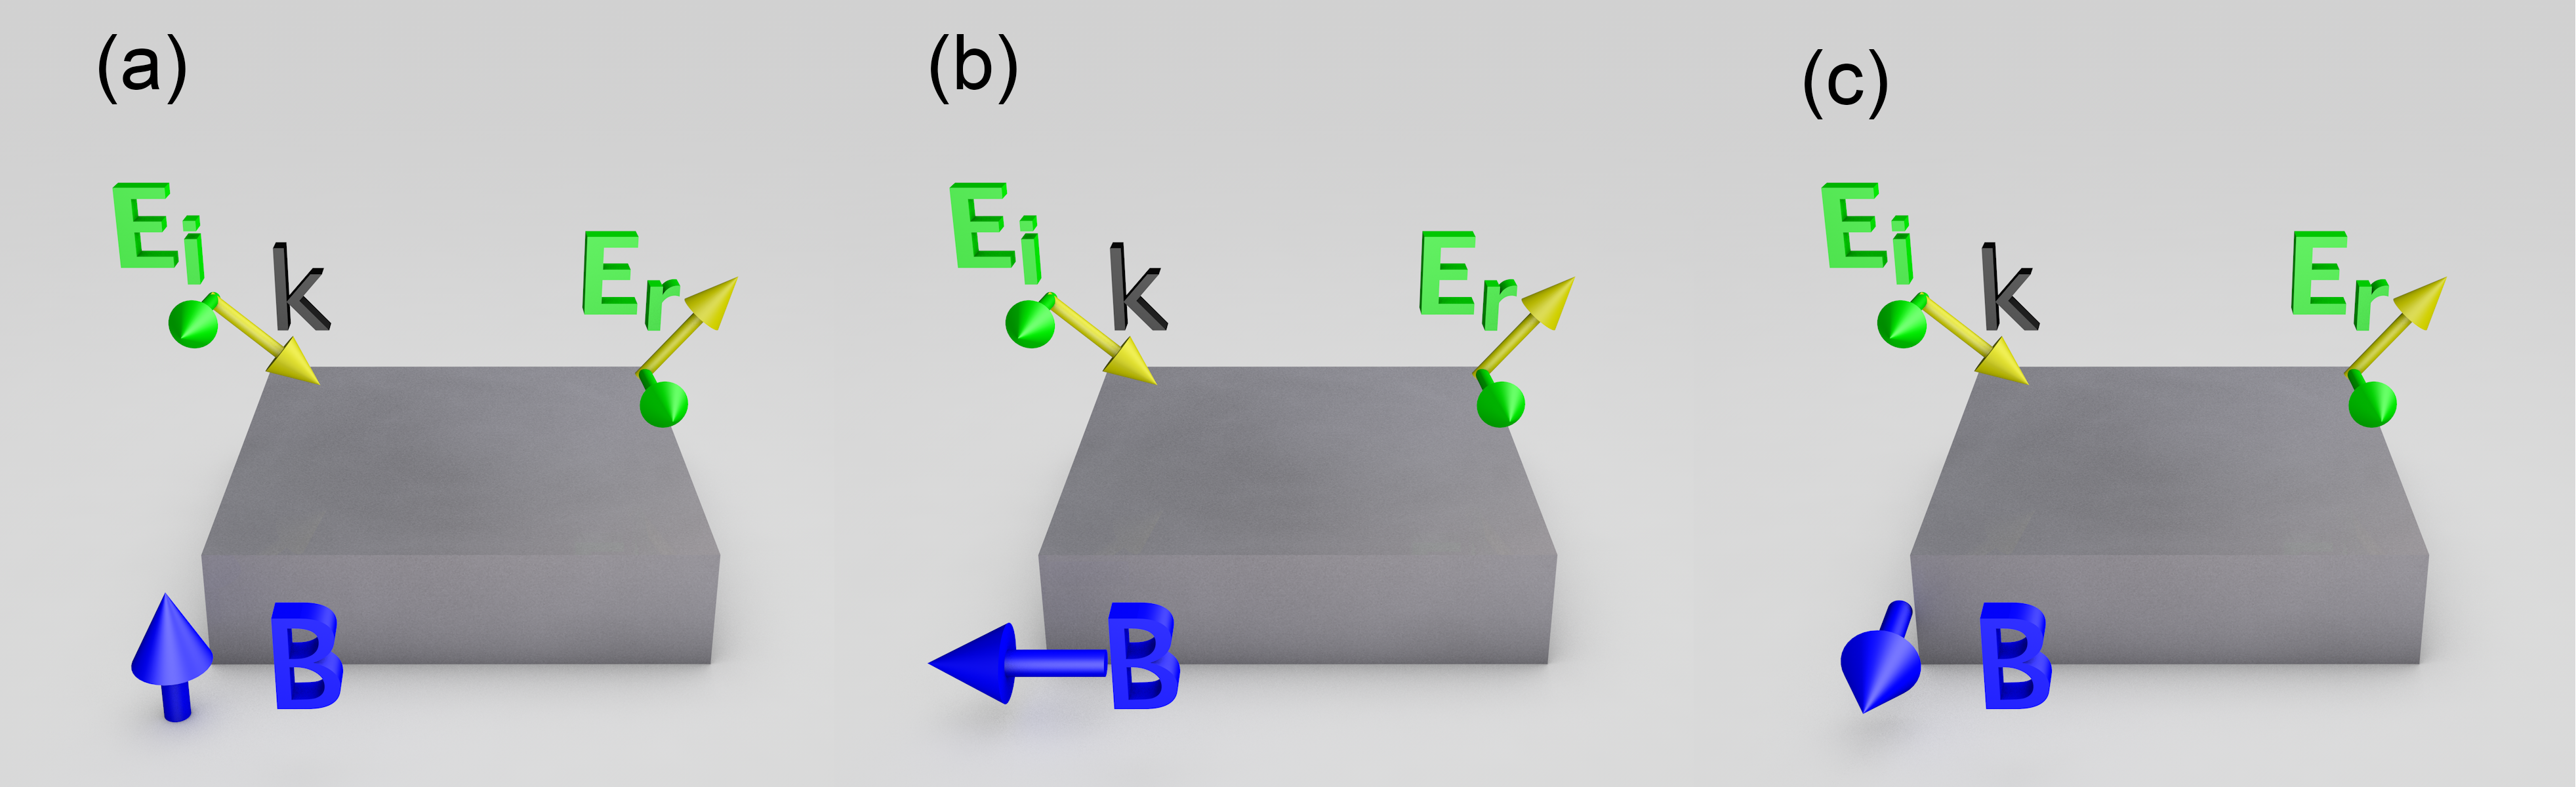
\includegraphics[width=12cm]{chapter_2/figures/kerr_configurations.png} 
\par\end{centering}
\caption{Schematic representation of the magneto-optical Kerr effect. In configuration: (a) is represented the polar configuration; (b) the longitudinal configuration; and (c) the transversal configuration. Each configuration is defined by the relative orientation between the magnetic field and the plane of incidence. \label{fig:chap2_kerr_config}}
\end{figure}



\section{Dipole radiation\label{chap2:Dipole_radiation}}

%In nature, many different types of structures, like atoms, molecules or quantum dots to name a few, radiate like dipoles. Such structures can be modelled as three level systems, with $\ket{e_{1}}$ and $\ket{e_{2}}$ two unstable vibrational levels of an excited electronic state and $\ket{g}$ the ground state. The system is excited with radiation at frequency $\omega_{e_{1}}$ to state $\ket{e_{1}}$ and instantly decay to the $\ket{e_{2}}$ state. At this point, it takes a time $\tau$ (lifetime) to jump to the fundamental state $\ket{g}$. This transition is followed by the emission of a photon at frequency $\omega_{e_{2}}$, called fluorescent frequency. \\

%\subsection{Purcell effect}

Since Purcell work in 1946 \cite{Purcell_1946}, it is known that the decay rate $\gamma$ (and consequently the lifetime $\gamma=\frac{1}{\tau}$) of an emitter is not only function of the intrinsic properties of atoms and molecules, but also of the environment where the emitter is placed.\\ 
 This phenomenon has been observed in emitters placed close to planar interfaces \cite{Drexhage_1966} and cavities \citep{Goy_1983}. Also it was theoretically predicted \cite{yablonovitch1987inhibited} and experimentally verified in two \cite{Kress_2005, Englund_2005} and three dimensional photonic crystals \cite{Lodahl_2004} and more recently in plasmonic \cite{Carminati_2006, Castanie_2012_distance, esteban2014strong} and magnetoplasmonic structures \cite{Nikolova_2013}.\\
A first approach to the understanding of this phenomenon can be made by evaluation the power radiated by an emitter when it is placed in different environments. Usually the modification of the radiated power is compared with the radiated power of the emitter in vacuum, \textit{i.e.}, in the absence of any scattering object.\\
In the following subsections we give a introduction to the analytical techniques to evaluate the radiated power, starting by calculate in free space and then in the presence of an inhomogeneous environment.

\subsection{Radiation in free space}

In the electromagnetic field, the representation of the energy flux density is given by the Poynting vector $\mathbf{S}$. This vector carries the information about the direction of propagation of the electromagnetic energy and is mathematically defined by:
\begin{equation}
\mathbf{S}\left(t\right)=\mathbf{E}\left(t\right)\times\mathbf{H}\left(t\right),
\end{equation} 
where the electric and magnetic field are in the time domain. For an electric point dipole $\boldsymbol{\mu}$, the radiated power can be determined by integrating the Poynting vector $\mathbf{S}\left(t\right)$ over a infinitesimally closed surface that surrounds the source. The average radiated power for an harmonically oscillating dipole is:

\begin{equation}
P_{0}=\frac{\left|\mathbf{\boldsymbol{\mu}}\right|^2}{4\pi\epsilon_{0}}\frac{k^4c}{3}.
\end{equation}
This equation indicates that the radiated power is proportional to the fourth power of the wavenumber.\\
An alternative way of evaluate the radiated power of a dipole in free space is presented in Appendix (\ref{App:eval_green_source}).
%As alternative, it could be calculated by integrating the time averaged P.

\subsection{Dipole radiation in inhomogeneous environments: \\ method I \label{subch:Dip_inh_envi}}

The behaviour of a dipole emitter embedded in an inhomogeneous environment can be characterised by the emitter radiated power. According with Poynting's theorem \cite{Jackson_CE}, the radiated power of a time harmonic current distribution is identical to the rate of energy dissipation:

\begin{equation}
\frac{dW}{dt}=-\frac{1}{2}\int_V^{} \Re\left\{\mathbf{j}^{*}\cdot\mathbf{E}\right\} dV.
\end{equation}
where $\mathbf{j}$ is not the total current density but instead represents the source current that generates the fields or the loss currents corresponding to the thermal losses and $V$ is the volume of the current distribution. If we consider the source like the one described in Eq. (\ref{eq:EM_source}), we obtain:


\begin{equation}
\left<\frac{dW}{dt}\right>=\frac{\omega}{2} \Im\left\{\boldsymbol{\mu}^{*}\cdot\mathbf{E}\left(\mathbf{r}_{0}\right)\right\},\label{eq:Radiated_power}
\end{equation}
being $\mathbf{E}\left(\mathbf{r}_{0}\right)$ the electric field at dipole position at $\mathbf{r}_0$.\\
In an inhomogeneous environment the field at dipole position $\mathbf{E}\left(\mathbf{r}_{0}\right)$ can be separated in two components. One is the dipole field in its own position $\mathbf{E}_{0}\left(\mathbf{r}_0\right)$ and the other is the scattered field  $\mathbf{E}_{s}\left(\mathbf{r}_0\right)$ by the surrounding environment. This can be expressed as:

\begin{equation}
\mathbf{E}\left(\mathbf{r}_{0}\right) = \mathbf{E}_{0}\left(\mathbf{r}_{0}\right) + \mathbf{E}_{s}\left(\mathbf{r}_{0}\right). \label{eq:E_source_inh}
\end{equation}
The total radiated power by the emitter can be evaluated by integrating the Poynting vector over the infinitesimal surface that surrounds the source. An alternative is to evaluate Eq. (\ref{eq:Radiated_power}) with an adequate field like Eq. (\ref{eq:E_source_inh}), \textit{i.e.}, the total electric field at the emitter position.\\
So, the total power radiated can be written as:

\begin{equation}
P_{tot}=\frac{\left|\mathbf{\boldsymbol{\mu}}\right|^2}{4\pi\epsilon_{0}}\frac{k^4c}{3} + \frac{kc}{2}\Im\left\{{\boldsymbol{\mu}^{*}\cdot \mathbf{E}_{s}\left(\mathbf{r}_{0}\right)}\right\}, 
\end{equation}
or normalized by the radiated power in free space:

\begin{equation}
\frac{P_{tot}}{P_{0}}=1 + \frac{6\pi\epsilon_{0}}{k^{3}\left|\boldsymbol{\mu}\right|^2}\Im\left\{{\boldsymbol{\mu}^{*}\cdot \mathbf{E}_{s}\left(\mathbf{r}_{0}\right)}\right\}\label{eq:norm_decay_rate}.
\end{equation}
From this equation we can see that the modification of the radiated power only depends of the scattered field, \textit{i.e.}, the field that returns after interfering with surroundings.

\subsection{Dipole radiation in inhomogeneous environments: \\ method II}

In an inhomogeneous environment like represented in Fig. (\ref{fig:inh_envir}), we can calculate the radiated power by an emitter in an alternative way to the one presented in Sec. (\ref{subch:Dip_inh_envi}).\\
The total radiated power by an emitter is obtained by evaluation of the radiated power in far field, which is called radiative power, and the absorbed power by the inhomogeneous environment. The first one, the radiated power in far field takes into account all the fields generated by the principal and secondary sources, formed by the emitter and the scattering particles respectively. The second one, the absorbed radiation by the inhomogeneous environment can be calculated by evaluating the absorbed power for all particles, like discussed in Sec. (\ref{sec:chap2_abs_small_part}). \\
Thus, due to the energy conservation:

\begin{equation}
P_{tot} = P_{rad} + P_{abs},
\end{equation}
where $P_{tot}$ is the total radiated power by the emitter, $P_{rad}$ is the radiated power by the entire system in far field and $P_{abs}$ the absorbed power by the environment. 

\begin{figure}[h]
\begin{centering}
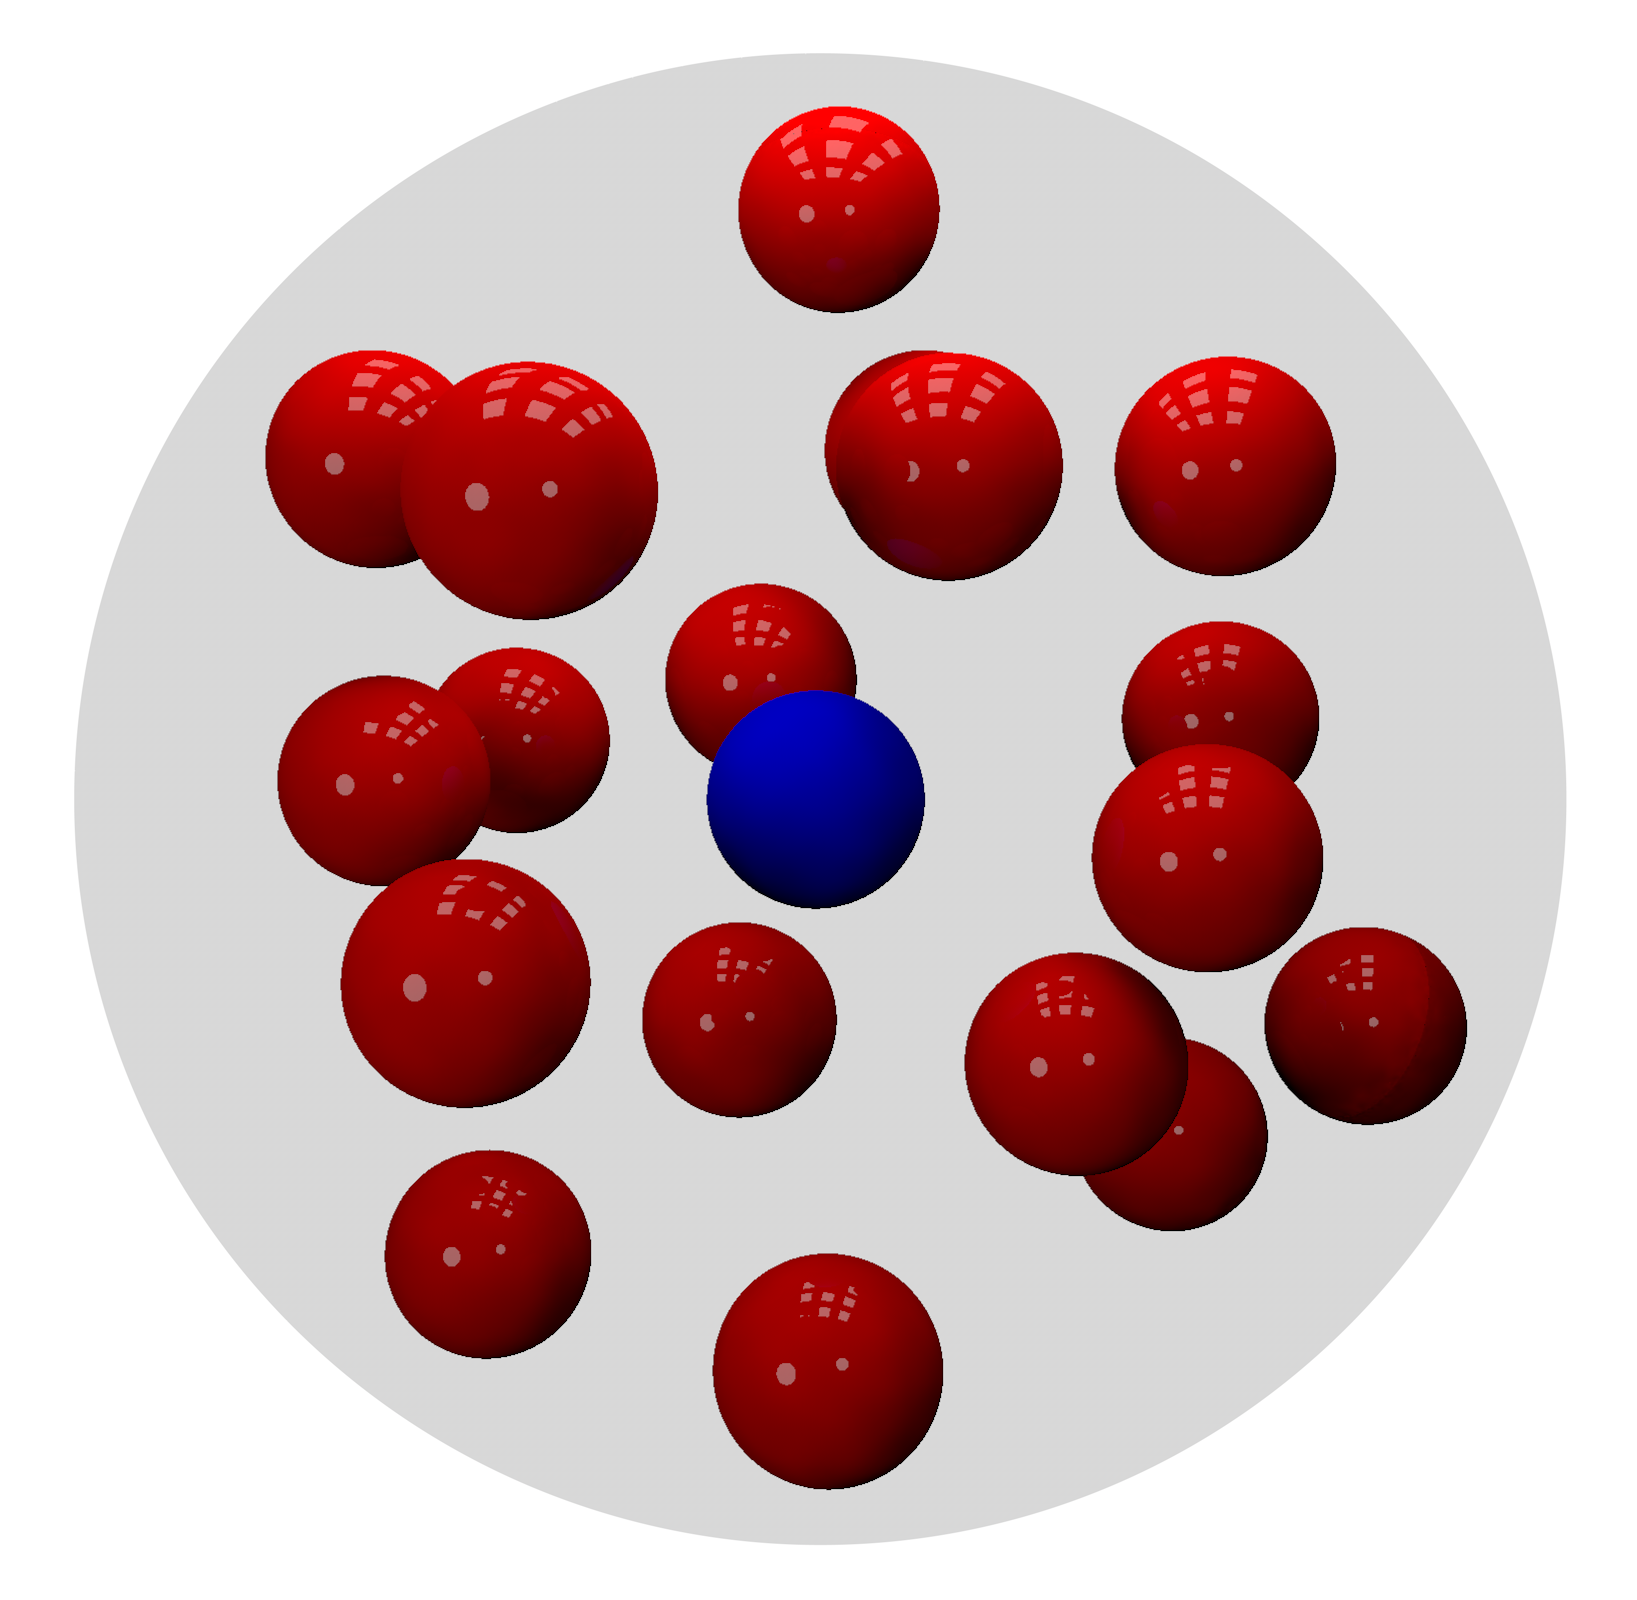
\includegraphics[width=6cm]{chapter_2/figures/inh_envirnm.png} 
\par\end{centering}
\caption{Schematic representation of an emitter $\boldsymbol{\mu}$ (blue sphere) in an inhomogeneous environment (represented by red spheres). The transparent sphere represents the shell that involves the entire system in far field.\label{fig:inh_envir}}
\end{figure}


Let us consider an emitter $\boldsymbol{\mu}$ located at $\mathbf{r} = \mathbf{r}_{0}$ surrounded by $\mathcal{N}$ dipolar particles $\mathbf{p}_n$ located at $\mathbf{r} = \mathbf{r}_{n}$ ($n = 1,...,\mathcal{N}$).

Considering the superposition principle, the total field at position $\mathbf{r}$ is given by:

\begin{equation}
\mathbf{E}\left(\mathbf{r}\right) = \frac{k^2}{\epsilon_{0}}\left[\mathbf{G}\left(\mathbf{r},\mathbf{r}_{0}\right)\cdot \boldsymbol{\mu} + \sum_{n=1}^{\mathcal{N}}\mathbf{G}\left(\mathbf{r},\mathbf{r}_{n}\right)\cdot \mathbf{p}_{n} \right].
\end{equation}

In far field, \textit{i.e.}, making the asymptotic expansion of the Green tensor $R = \left|\mathbf{r}\right| \gg \left|\mathbf{r}_{n}\right|$, and $\mathbf{k}$ the wave vector defined by $\mathbf{k}=k \mathbf{u}_{r}$ with $\mathbf{u}_{r}={\mathbf{r}}/{\left|\mathbf{r}\right|}$, the electric and magnetic field can be written as:

\begin{eqnarray}
\mathbf{E}_{n}\left(\mathbf{r}\right) & = & \frac{k^{2}}{\epsilon_{0}}\mathbf{G}\left(\mathbf{r},\mathbf{r}_{n}\right)\cdot\mathbf{p}_{n}\approx\frac{e^{ikR}}{4\pi\epsilon_{0}} R \left\{ \left(\mathbf{k}\times\mathbf{p}_{n}\right)\times\mathbf{k}\right\} e^{-i\mathbf{k}\cdot\mathbf{r}_{n}}\\
\mathbf{H}_{n}\left(\mathbf{r}\right) & = & \frac{1}{k}\sqrt{\frac{\epsilon_{0}}{\mu_{0}}}\left(\mathbf{k}\times\mathbf{E}_{n}\right).
\end{eqnarray}


With the electric and magnetic field is defined the Poynting vector. Integrating over a spherical surface that contains the entire system (see App. (\ref{App1:eval_dip_inh_env})), the total radiated power will be given by:
\begin{equation}
P = \frac{k^3}{2}\frac{1}{\epsilon_{0}\sqrt{\epsilon_{0} \mu_{0}}} \sum_{mn}\Re \left\{ \mathbf{p}_{m}^{*}\cdot \Im \left[ \mathbf{G} \left(\mathbf{r}_{m},\mathbf{r}_{n}\right)\right]\cdot \mathbf{p}_{n} \right\}.
\end{equation} 


\subsection{Local Density of states (LDOS)}

When an emitter is embedded in an inhomogeneous environment, the radiated power is a function of its position, orientation and frequency. It also possess an angular distribution determined by the modal structure and the number of available electromagnetic fields at the position of the emitter, the so called density of electromagnetic states. Due to the nature of some problems, in particular the ones addressed in this thesis, the density of states is evaluated depending on the position, called local density of states (LDOS).

Experimentally it can be evaluated by measuring the lifetime of an emitter positioned at the point under study.
In cases where the orientation of the transition dipole is not well defined, the decay rate is averaged over the various orientations.

The local density of states is obtained by the imaginary part of the Green tensor:

\begin{equation}
\rho\left(\mathbf{r},\omega\right) = \frac{2\omega}{\pi c^2}\Im{\left\{Tr\left[\mathbf{G}\left(r,r,\omega\right)\right]\right\}}.
\end{equation}

This quantity is directly related with the spontaneous decay rate of an emitter averaged over its dipole orientation $\mathbf{n}$:

\begin{equation}
\left<\Gamma\right>_{\mathbf{n}}=\frac{\omega\pi}{3\epsilon_{0}\hbar}\left|\mathbf{p}\right|^2\rho\left(\mathbf{r},\omega\right).
\end{equation}

where $\left<.\right>_{\mathbf{n}}$ is the average over the dipole orientation, $\mathbf{p}$ is the transition dipole of the emitter and $\hbar$ is the reduced Planck constant.




%To understand the behavior of a dipole emitter embedded in an inhomogeneous environment we should look carefully to the rate of energy dissipation given by \cite{Jackson_CE}:


\section{Summary}

In this chapter we summarise the fundamental tools used in the following chapters.\\ 
We have introduced a classical formalism that describes the interaction of nanosystems characterised by their polarisabilities and an electromagnetic field. \\
Detailed discussions of the electromagnetic theory can be found in general textbooks \cite{Jackson_CE,stratton2007electromagnetic,landau1975classical,born1999principles, van2007electromagnetic}. More oriented books on scattering theory can be found in references \cite{bohren2008absorption, nieto2006scattering,Ping:2006kn}. A recent book with an interesting approach to nano-optics can found in reference \cite{Novotny_PNO_2012}.


%
%
%
%
%
%
%
%End of chapter
%
%

